% 
\chapter{Implementação da Solução} 
\label{chap:Impl}

A fase de implementação/desenvolvimento de software segue as diretrizes definidas na análise e no design do sistema, traduzindo-as em código-fonte e linguagem de programação \cite{UBIMINDS2025}. É nesta etapa que se integram sistemas externos e se utilizam ferramentas que auxiliam na programação, rastreio de código, colaboração da equipa, gestão de tarefas e cumprimento de prazos e metas estabelecidos.

Neste capítulo, será descrito o processo de implementação do projeto ao longo de várias fases, nomeadamente as fases de planeamento e de desenvolvimento. Serão também referidas as tecnologias utilizadas, incluídas imagens representativas da plataforma criada e explicadas as funcionalidades implementadas, conforme definidas nos casos de uso apresentados nos Capítulos \ref{chap:AP} e \ref{chap:DS}. Detalhes considerados desnecessários para a compreensão do trabalho serão remetidos para os anexos.

%-------------------------------------------------------------------------------

\section{Descrição da implementação} 
\label{sec:desc}

\subsection{Tecnologias Usadas}

Nesta subsecção são descritas as tecnologias usadas na implementação, categorizadas entre pré-desenvolvimento, referentes ao planeamento desta fase, e desenvolvimento, relativamente à implementação da solução.

\subsubsection{Tecnologias de Pré-desenvolvimento}

No desenvolvimento dos diagramas da vista de progresso (Subsecção \ref{subsec:process_view}) que servem de guia para a implementação das funcionalidades foi usado o \textit{PlantUML}\footnote{Site do \textit{Plantuml}: \url{https://plantuml.com/}} compilado no \textit{Visual Studio Code}\footnote{Site do \textit{Visual Studio Code}: \url{https://code.visualstudio.com/}}. Os restantes diagramas foram feitos pelo programa \textit{Draw.io}\footnote{Site do \textit{Draw\.io}: \url{https://www.drawio.com/}}.

O protótipo da plataforma \gls{ESG}, referido no Apêndice \ref{AppendixC}, foi realizado no \textit{Figma}\footnote{Site do \textit{Figma}: \url{https://www.figma.com/}}, a divisão de tarefas e planeamento do projeto foi realizado no \textit{Github Projects}\footnote{Página sobre o \textit{Github Projects}: \url{https://docs.github.com/en/issues/planning-and-tracking-with-projects/learning-about-projects/about-projects}}, como ilustrado na Figura \ref{fig:kanbanBoard}, e o repositório foi alocado no \textit{Github}\footnote{Site do \textit{Github}: \url{https://github.com/}}. A aplicação tem como referência visual o \textit{kit} de marca da Devscope\footnote{Site do \textit{kit} de marca da Devscope: \url{https://brand.devscope.net/intro.html}}

\begin{figure}[H]
    \centering
    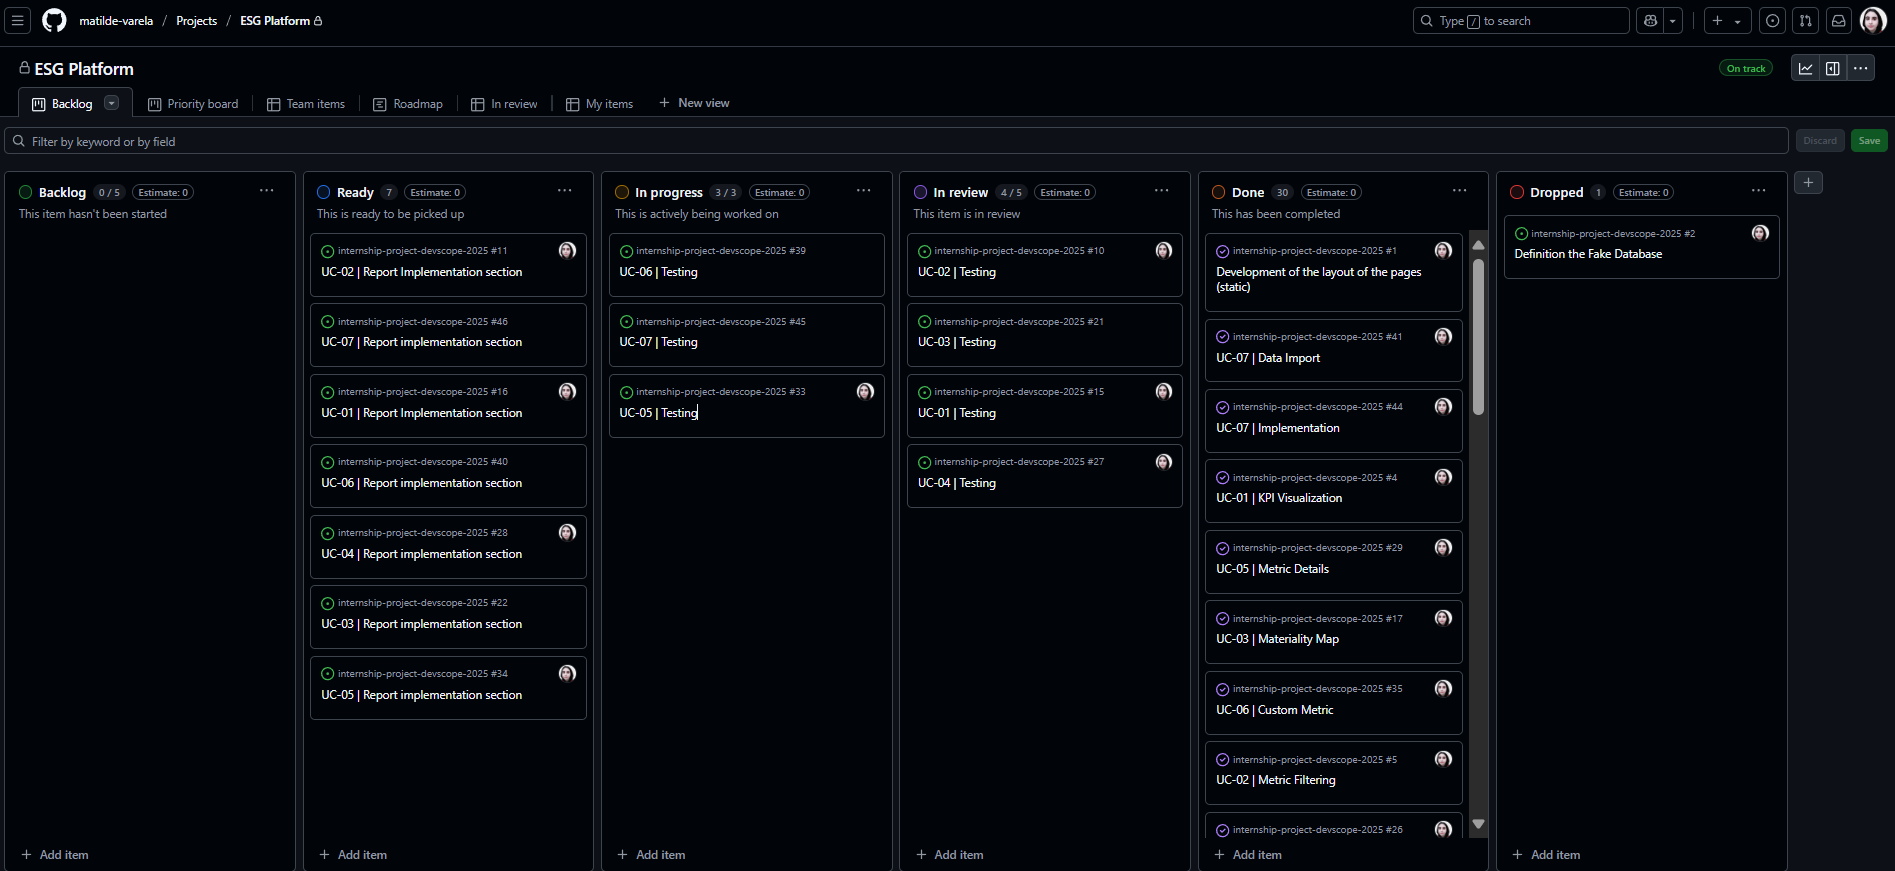
\includegraphics[width=\linewidth,keepaspectratio]{frontmatter/assets/github_projects.png}
    \caption{Painel com quadro \textit{kanban} usado no planeamento do projeto}
    \label{fig:kanbanBoard}
\end{figure}

\subsubsection{Tecnologias de Desenvolvimento}

Relativamente às tecnologias utilizadas no desenvolvimento do projeto, o \textit{Visual Studio Code} foi o editor escolhido para a escrita do código-fonte.

No que diz respeito ao \textit{frontend}, recorreu-se ao \textit{TypeScript} como linguagem de programação de alto nível, de código aberto\footnote{Site oficial do \textit{TypeScript}: \url{https://www.typescriptlang.org/}}. O \textit{TypeScript} é uma versão melhorada do \textit{JavaScript}, orientada a objetos, sendo preferida em projetos de maior escala devido à sua robustez, melhor manutenção e escalabilidade.

Para o desenvolvimento da interface, utilizaram-se as tecnologias \textit{React}\footnote{Site do \textit{React}: \url{https://react.dev/}}, uma biblioteca \textit{JavaScript} focada na construção de interfaces de utilizador, especialmente em aplicações do tipo \gls{SPA}, e \textit{Next.js}\footnote{Site do \textit{Next.js}: \url{https://nextjs.org/}}, uma \textit{framework} baseada em \textit{React} que facilita a criação de aplicações web com funcionalidades como renderização no lado do servidor (\textit{Server-Side Rendering}) e geração estática de páginas.

A nível de estilização, foi usada a \textit{framework} \textit{Tailwind CSS}\footnote{Site do \textit{Tailwind CSS}: \url{https://tailwindcss.com/}}, que permite desenvolver rapidamente interfaces personalizadas através da aplicação de classes utilitárias diretamente no HTML, evitando a necessidade de escrever folhas de estilo tradicionais.

No \textit{frontend}, foi utilizado o \textit{Vuexy}\footnote{Site oficial: \url{https://pixinvent.com/vuexy-bootstrap-html-admin-template/}} como base para o desenvolvimento do painel de administração. Este \textit{template} de \textit{dashboard} é altamente personalizável e compatível com tecnologias como \textit{Vue.js}\footnote{Site oficial: \url{https://vuejs.org/}}, \textit{React}, \textit{HTML} e \textit{Laravel}\footnote{Site oficial: \url{https://laravel.com/}}, oferecendo componentes reutilizáveis, gráficos e estruturas de layout. Para a visualização interativa dos dados, foi utilizada a biblioteca \textit{ApexCharts}\footnote{Site oficial: \url{https://apexcharts.com/}}, uma solução \textit{open source} baseada em \textit{JavaScript}.

A escolha de todas as tecnologias mencionadas foi uma exigência da empresa onde decorreu o estágio, assegurando a compatibilidade do projeto desenvolvido com os restantes produtos e soluções da organização.

A plataforma \textit{Railway}\footnote{Site oficial: \url{https://railway.com/}} foi utilizada para alojar a base de dados relacional \textit{MySQL}\footnote{Site oficial: \url{https://www.mysql.com/}} e realizar o \textit{deployment} da aplicação. Esta permite integração direta com repositórios \textit{Git}, facilitando a integração contínua e a publicação. Para além disso, trata automaticamente da infraestrutura e escalabilidade, sendo útil no desenvolvimento e manutenção de aplicações \textit{web}.

Para o armazenamento de ficheiros estáticos, como imagens associadas às métricas ESG, foi utilizado o serviço da \textit{Amazon} \textit{AWS S3}\footnote{Site do \textit{AWS S3}: \url{https://aws.amazon.com/s3/}}, onde foi criado um \textit{bucket} próprio para o projeto. As imagens são alojadas nesse \textit{bucket}, sendo o respetivo URL público guardado no atributo \texttt{imageURL} da tabela de métricas ESG da base de dados \textit{MySQL}. 

A interação com a base de dados foi facilitada pelo uso do \textit{Prisma}\footnote{Site do \textit{Prisma}: \url{https://www.prisma.io/}}, uma ferramenta ORM (\textit{Object-Relational Mapping}) que permite definir o esquema da base de dados de forma declarativa, através de um ficheiro \texttt{schema.prisma}. Para além disso, o \textit{Prisma} foi utilizado na criação de \textit{scripts} de \textit{seeding}, que permitem inserir dados fictícios na base de dados, e também para a limpeza e eliminação de dados durante o processo de desenvolvimento.

\section{Funcionalidades}

\subsection{Página Inicial | \textit{Dashboard}}

A página inicial, Figura \ref{fig:homepage}, apresenta a informação mais recente e dinâmica da plataforma, incluindo a pontuação ESG e os principais KPI's. Esta implementação abrange os casos de uso UC-01 (Visualização de KPI's) e UC-04 (Pontuação ESG), destacando as métricas que registaram melhorias ou quedas em relação ao valor anterior.

\begin{figure}[H]
    \centering
    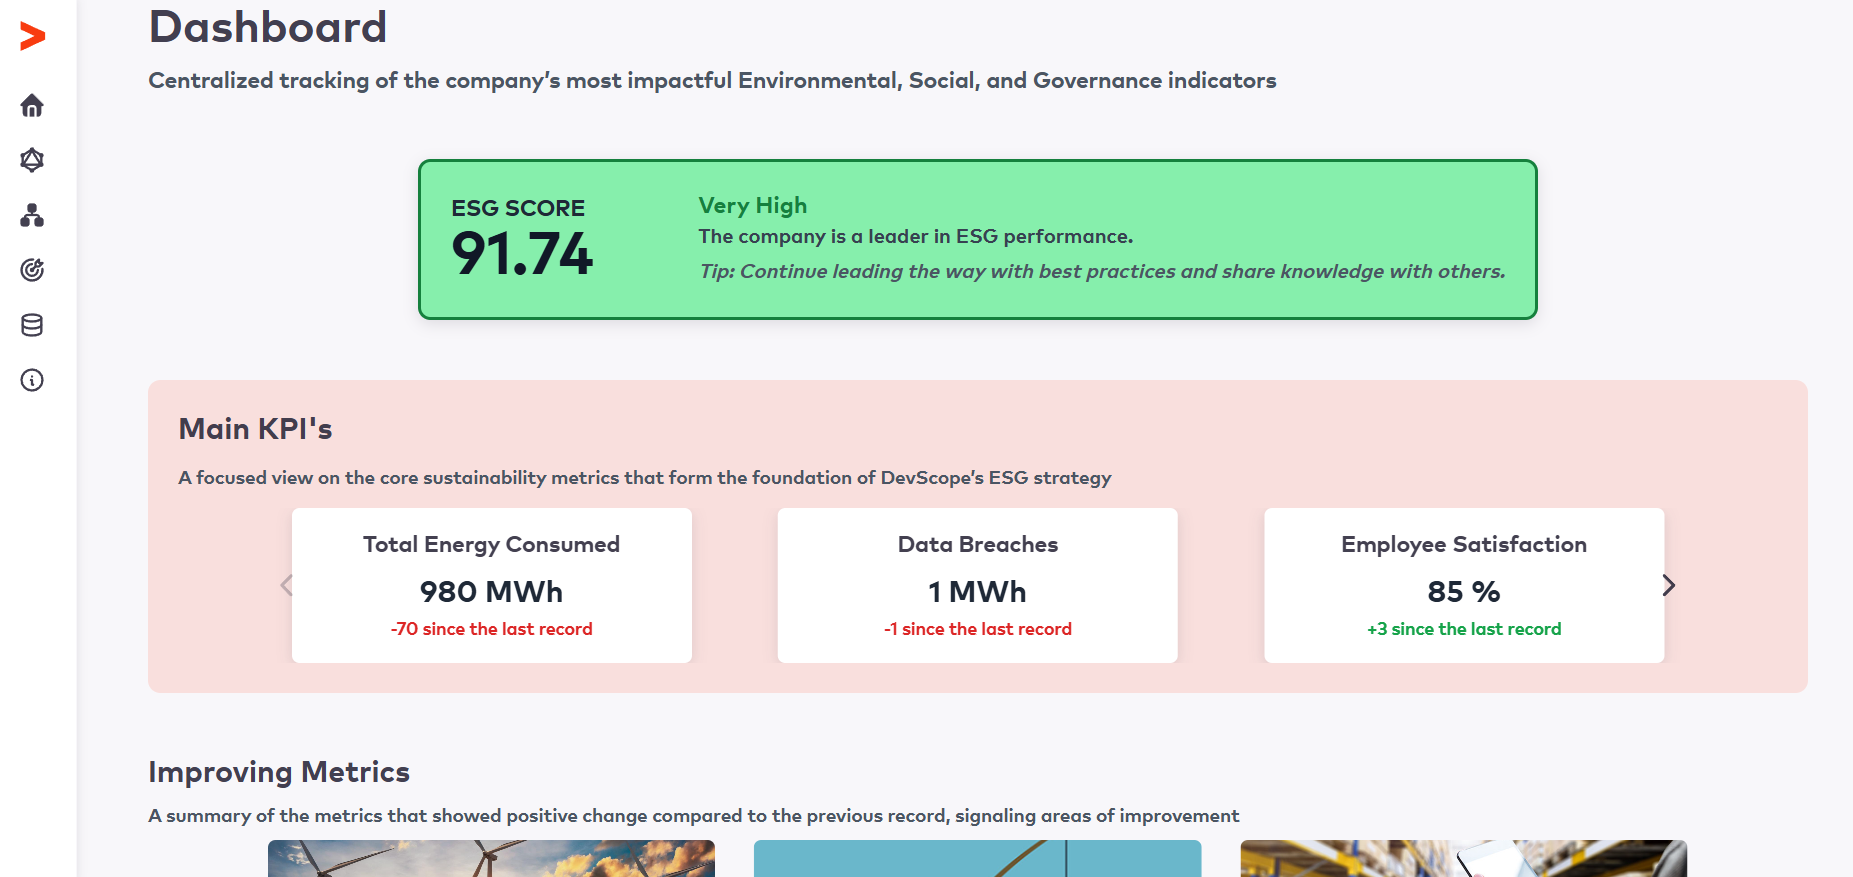
\includegraphics[width=\linewidth,keepaspectratio]{frontmatter/assets/platform_prints/dashboard/dashboard_done.png}
    \caption{Página Inicial com pontuação ESG}
    \label{fig:homepage}
\end{figure}

O valor obtido na pontuação ESG surge de uma fórmula criada com base no artigo redigido por \cite{Berg2022}, que explora as divergências das várias metodologias para classificações ESG usadas pelas agências na classificação do desempenho ESG das empresas. Tendo em conta o conteúdo do artigo, uma nova fórmula foi desenvolvida. A pontuação ESG é calculada através de uma abordagem hierárquica que agrega métricas em subáreas, subáreas em pilares, e finalmente combina os pilares para obter a pontuação final. O processo segue as seguintes etapas:

\textbf{Normalização de Métricas}

Cada métrica é normalizada para uma escala de 0 a 100 ao utilizar os seus valores mínimo e máximo definidos:

\begin{equation}
    \text{valor\_normalizado} = \begin{cases}
        \frac{\text{valor\_bruto} - \text{minValue}}{\text{maxValue} - \text{minValue}} \times 100 & \text{se minValue e maxValue existirem} \\
        \text{valor\_bruto} & \text{caso contrário}
    \end{cases}
\end{equation}

\textbf{Cálculo de Pontuação por Subárea}

Para cada subárea, calcula-se a média das métricas ativas (com \textit{activationStatus} verdadeiro) e aplica-se o peso da subárea:

\begin{equation}
    \text{pontuação\_subarea} = \left( \frac{\sum_{i=1}^{n} \text{valor\_normalizado}_i}{n} \right) \times \text{peso\_subarea}
\end{equation}

onde $n$ é o número de métricas ativas na subárea.

\textbf{Cálculo de Pontuação por Pilar}

A pontuação de cada pilar é calculada como a média ponderada das subáreas pertencentes a esse pilar:

\begin{equation}
    \text{pontuação\_pilar} = \left( \frac{\sum_{j=1}^{m} \text{pontuação\_subarea}_j}{\sum_{j=1}^{m} \text{peso\_subarea}_j} \right) \times \text{peso\_pilar}
\end{equation}

onde $m$ é o número de subáreas no pilar.

\textbf{Cálculo da Pontuação ESG Final}

A pontuação final ESG é obtida pela média ponderada dos pilares, limitada ao intervalo [0, 100]:

\begin{equation}
    \text{pontuação\_final} = \min\left(100, \max\left(0, \frac{\sum_{k=1}^{p} \text{pontuação\_pilar}_k}{\sum_{k=1}^{p} \text{peso\_pilar}_k}\right)\right)
\end{equation}

onde $p$ é o número total de pilares considerados (Ambiental, Social e Governança).

No \textit{frontend}, os dados do \textit{dashboard} são obtidos dinamicamente através de uma chamada HTTP do tipo \texttt{GET}, utilizando a função \texttt{fetch} (Listagem~\ref{lst:fetch_dashboard}) para aceder à rota \texttt{/api/dashboard}. A resposta, em formato JSON, agrega todas as métricas necessárias, evitando múltiplas chamadas à API e melhorando a performance da aplicação.

\begin{lstlisting}[style=customts, caption={Função responsável por obter os dados do ESG Score e do dashboard no carregamento do componente}, label={lst:fetch_dashboard}]
 useEffect(() => {
    document.title = `Dashboard | ESG Platform`;
    const fetchData = async () => {
      try {
        const responseScore = await fetch('/api/esgScore');
        if (!responseScore.ok) {
          throw new Error('Failed to fetch ESG score');
        }
        const dataScore = await responseScore.json();
        console.log('data score esg ', dataScore)
        setEsgScore(dataScore);
        setCategory(classifyESGScore(dataScore));
        const responseData = await fetch('/api/dashboard');
        if (!responseData.ok) {
          throw new Error('Failed to fetch dashboard info');
        }
        const dashboardData = await responseData.json();
        setKPIs(dashboardData.kpis);
        setBestN(dashboardData.bestMetrics);
        setWorstN(dashboardData.worstMetrics);
      } catch (err: any) {
        setError(err.message);
      } finally {
        setIsLoading(false);
      }
    };
    fetchData();
  }, []);
\end{lstlisting}

De modo a melhorar a experiência do utilizador relativamente à espera do retorno da informação requisitada foi desenvolvido um excerto HTML (Listagem \ref{lst:loading_code}) que escure-se levemente a plataforma e introduz um componente circular a indicar o progresso de obtençao das informaçoes.

\begin{lstlisting}[style=customts, caption={Componente mostrado no carregamento da página}, label={lst:loading_code}]
  if (isLoading) {
    return (
      <Backdrop
        open={true}
        sx={{
          backgroundColor: 'rgba(255, 255, 255, 0.7)',
          zIndex: (theme) => theme.zIndex.modal + 1,
          display: 'flex',
          flexDirection: 'column',
          gap: 2
        }}
      >
        <CircularProgress color="primary" size={60} />
      </Backdrop>
    )
  }
\end{lstlisting}

O mesmo foi feito caso acontecesse algum erro, como demonstrado na Listing \ref{lst:error_code}.

\begin{lstlisting}[style=customts, caption={Componente mostrado no caso de erro no carregamento da página}, label={lst:error_code}]
  if (error) {
    return (
      <Dialog open={true}>
        <DialogTitle>Error</DialogTitle>
        <DialogContent>
          <div style={{ color: 'red', padding: '16px' }}>
            Error: {error}
          </div>
        </DialogContent>
        <DialogActions>
          <Button onClick={() => setError(null)}>Close</Button>
        </DialogActions>
      </Dialog>
    )
  }
\end{lstlisting}

Os KPIs apresentam os valores atuais das métricas classificadas como tal, assim como a sua evolução desde o último registo. Esta variação é destacada com um código de cores: verde para evolução positiva e vermelho para desempenho negativo.

A distinção entre as melhores e piores métricas é feita com base na evolução das métricas ativas (com \textit{activationStatus} verdadeiro), calculada entre o primeiro e o último valor registado. O delta obtido determina a inclusão da métrica no conjunto das cinco melhores ou cinco piores.

\subsection{Página das Métricas}

Esta página (Figura \ref{fig:metric_done}) da plataforma agrupa várias informações e funcionalidades, nomeadamente as que são referentes aos casos de uso UC-05 (Visualização dos detalhes das métricas), UC-02 (Filtragem de métricas), e UC-06 (Métricas Customizáveis).

\begin{figure}[H]
    \centering
    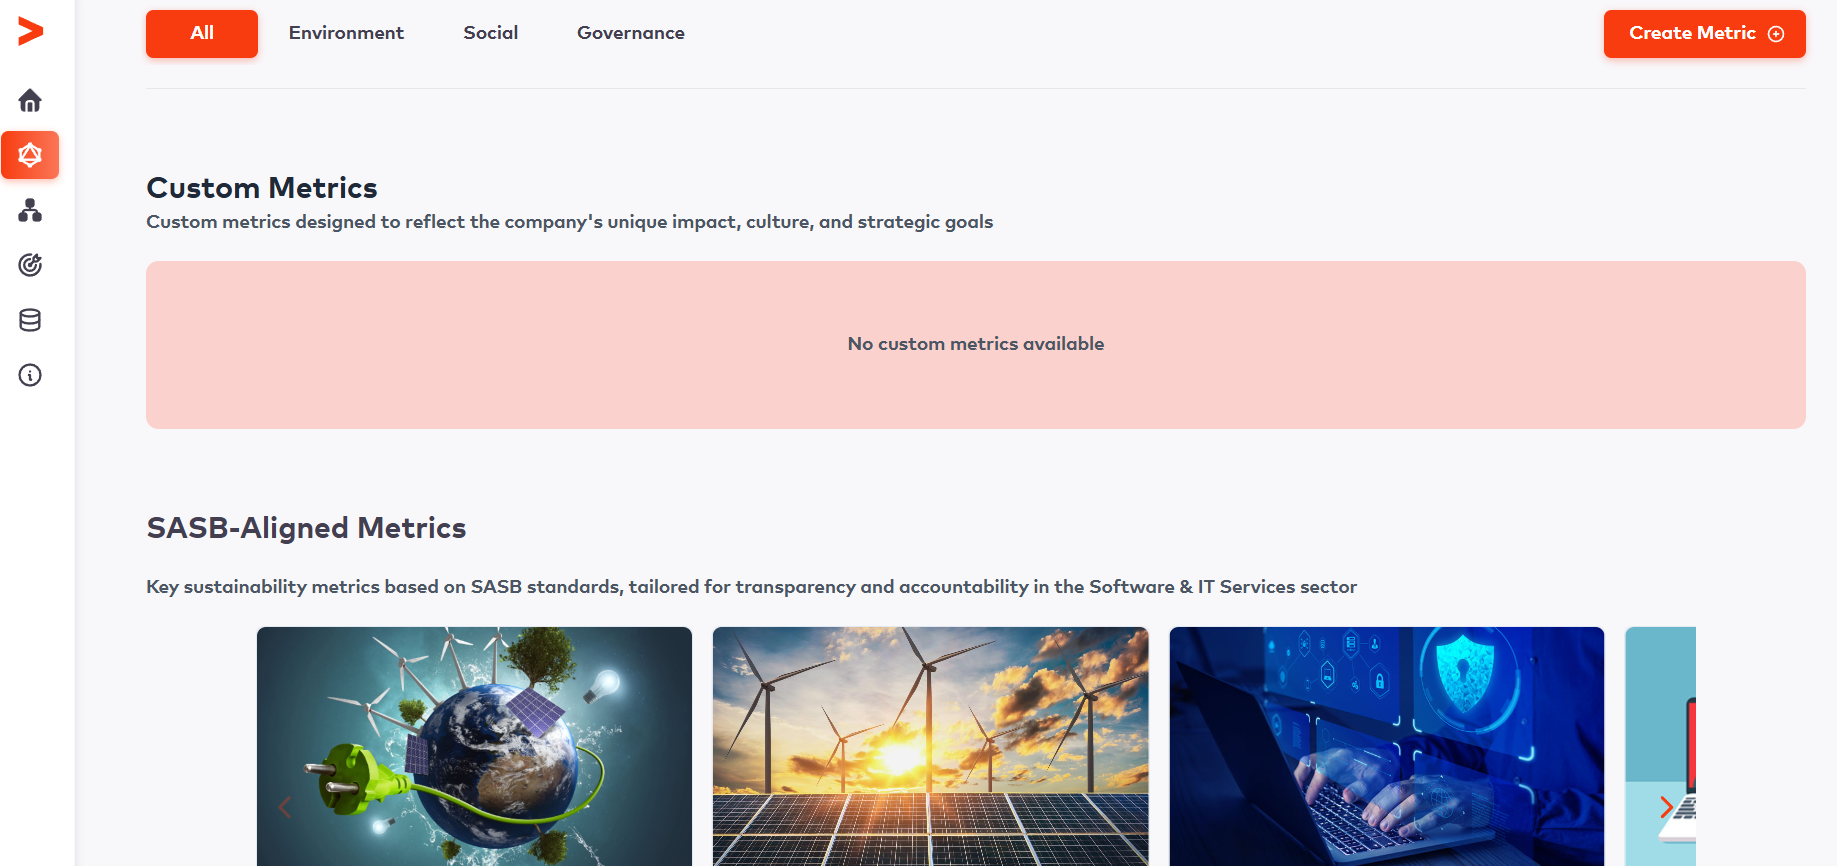
\includegraphics[width=\linewidth,keepaspectratio]{frontmatter/assets/platform_prints/metrics/metrics_done.png}
    \caption{Página das Métricas}
    \label{fig:metric_done}
\end{figure}

A interface da aplicação apresenta um conjunto de separadores (\textit{tabs}) que representam os diferentes pilares ESG, funcionando como mecanismo de filtragem das métricas (UC-02). Por defeito, todos os pilares estão selecionados, permitindo visualizar a totalidade das métricas disponíveis. A Listagem \ref{lst:metric_filter} ilustra a lógica de filtragem implementada: caso o valor de \texttt{selectedPillar} seja \texttt{'All'}, são apresentadas todas as métricas; caso contrário, apenas são consideradas as métricas associadas ao pilar selecionado.

\begin{lstlisting}[style=customts, caption={Excerto de Código com Filtragem das Métricas}, label={lst:metric_filter}]
const filteredMetrics = useMemo(() => {
return selectedPillar === 'All'
    ? metrics
    : metrics.filter((metric) => metric.subarea?.pillar?.name === selectedPillar)
}, [metrics, selectedPillar])
\end{lstlisting}

Adicionalmente, é feita uma distinção clara entre as métricas definidas pela framework \gls{SASB}, específicas para o setor de \textit{Software} e Serviços IT, e as métricas personalizadas criadas pela empresa (UC-06). Esta criação é realizada através de um \textit{popup}, ilustrado na Figura \ref{fig:metric_creation}, permitindo adaptar a plataforma às necessidades da organização. As informações submetidas são enviadas via API e armazenadas na base de dados.

\begin{figure}[H]
    \centering
    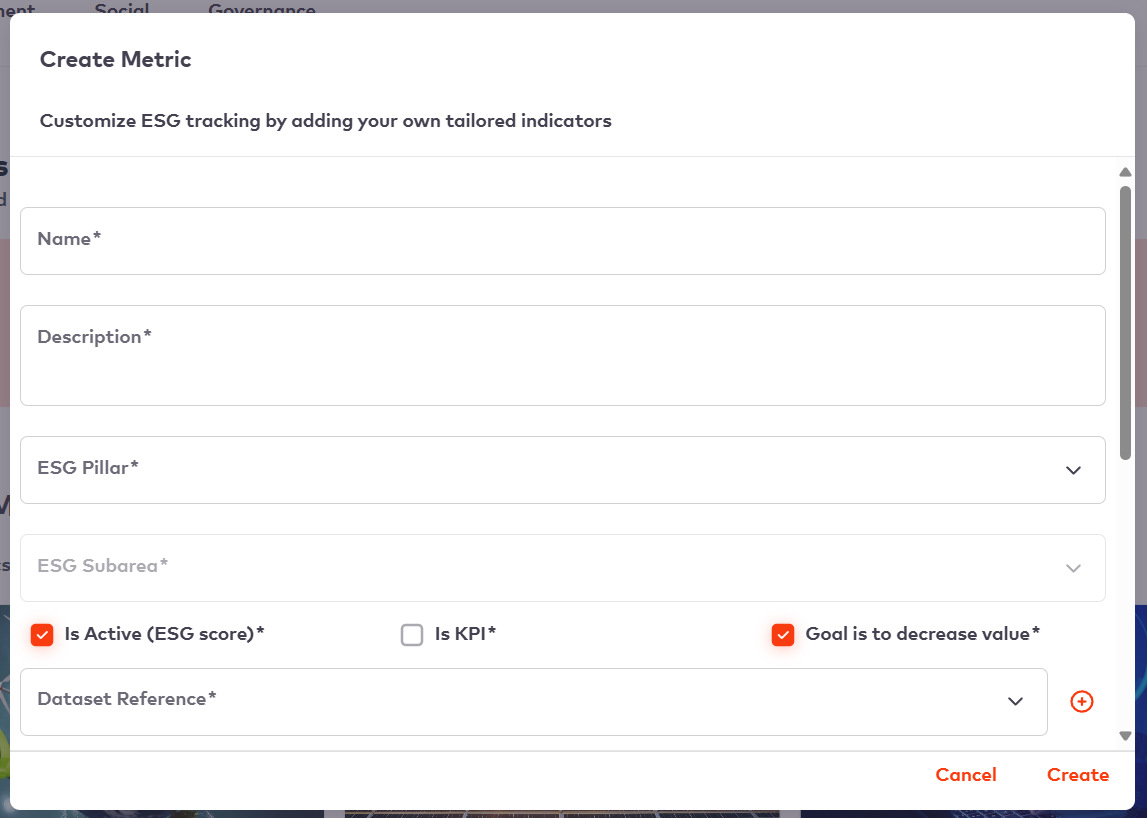
\includegraphics[width=5in,keepaspectratio]{frontmatter/assets/platform_prints/metrics/metric_creation.png}
    \caption{Formulário de Criação de Métrica}
    \label{fig:metric_creation}
\end{figure}

Tendo em conta que cada métrica está relacionada com uma imagem e que o armazenamento de imagens como BLOB em bases de dados não é aconselhável, por questões de desempenho e escalabilidade, foi implementada uma solução híbrida (\cite{code-examplesnet2025}). As imagens são armazenadas no serviço AWS S3, que é perfeito para ficheiros estáticos, e o URL gerado é guardado na base de dados, com o objetivo de ser utilizado na renderização do cartão da métrica (Listagem \ref{lst:image_upload}).

\begin{lstlisting}[style=customts, caption={Função de \textit{Upload} de uma imagem para o AWS S3}, label={lst:image_upload}]
export async function generateSignedUploadUrl(fileName: string, fileType: string) {
  const key = `${folder}/${fileName}`
  const command = new PutObjectCommand({
    Bucket: bucket,
    Key: key,
    ContentType: fileType,
  })
  const url = await getSignedUrl(s3, command, { expiresIn: 60 })
return { url, key, bucket }
}
\end{lstlisting}

Cada cartão representante de uma métrica é interativo. Quando clicado, abre uma janela com as informações da métrica (UC-05), como ilustrado pela Figura \ref{fig:metric_info}. Esta janela mostra os diferentes atributos das metricas.

\begin{figure}[H]
    \centering
    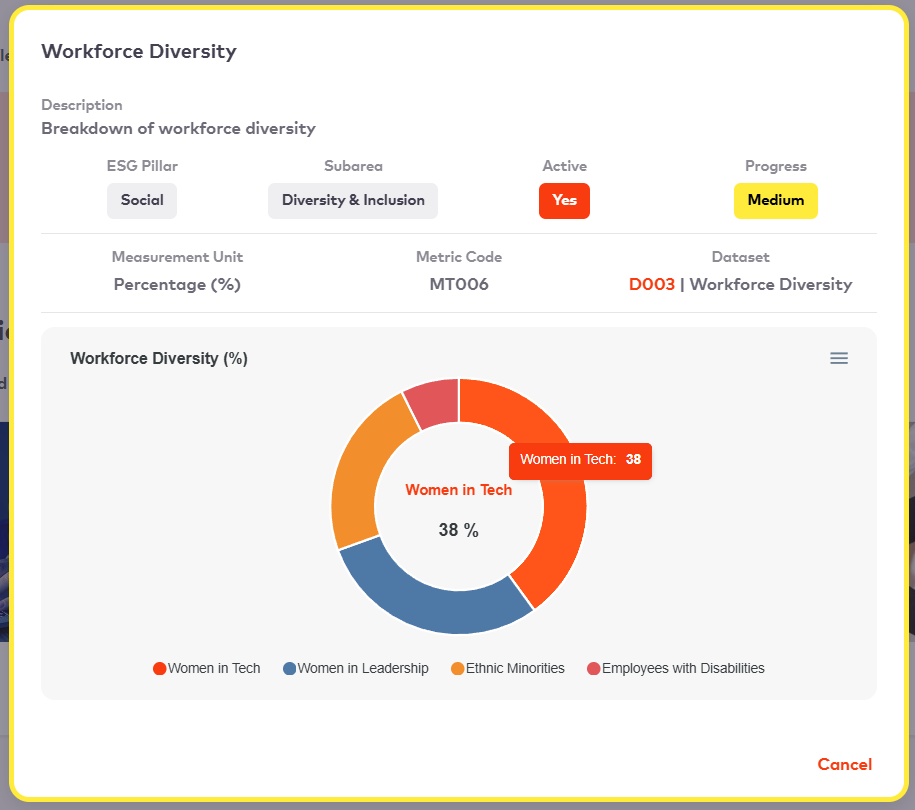
\includegraphics[width=5.5in,keepaspectratio]{frontmatter/assets/platform_prints/metrics/metric_info.png}
    \caption{Cartão com informação detalhada da Métrica}
    \label{fig:metric_info}
\end{figure}

\subsection{Mapa de Materialidade}

O mapa de materialidade, abordado no Capítulo \ref{chap:EA}, corresponde a uma matriz que agrega as métricas consideradas relevantes para a avaliação ESG da empresa. A plataforma apresenta este elemento numa página dedicada, Figura \ref{fig:matrix_done}, organizada por pilares, subáreas e métricas ativas. O objetivo é fornecer uma visualização clara das áreas cujo progresso ainda se encontra aquém do desejável.

\begin{figure}[H]
    \centering
    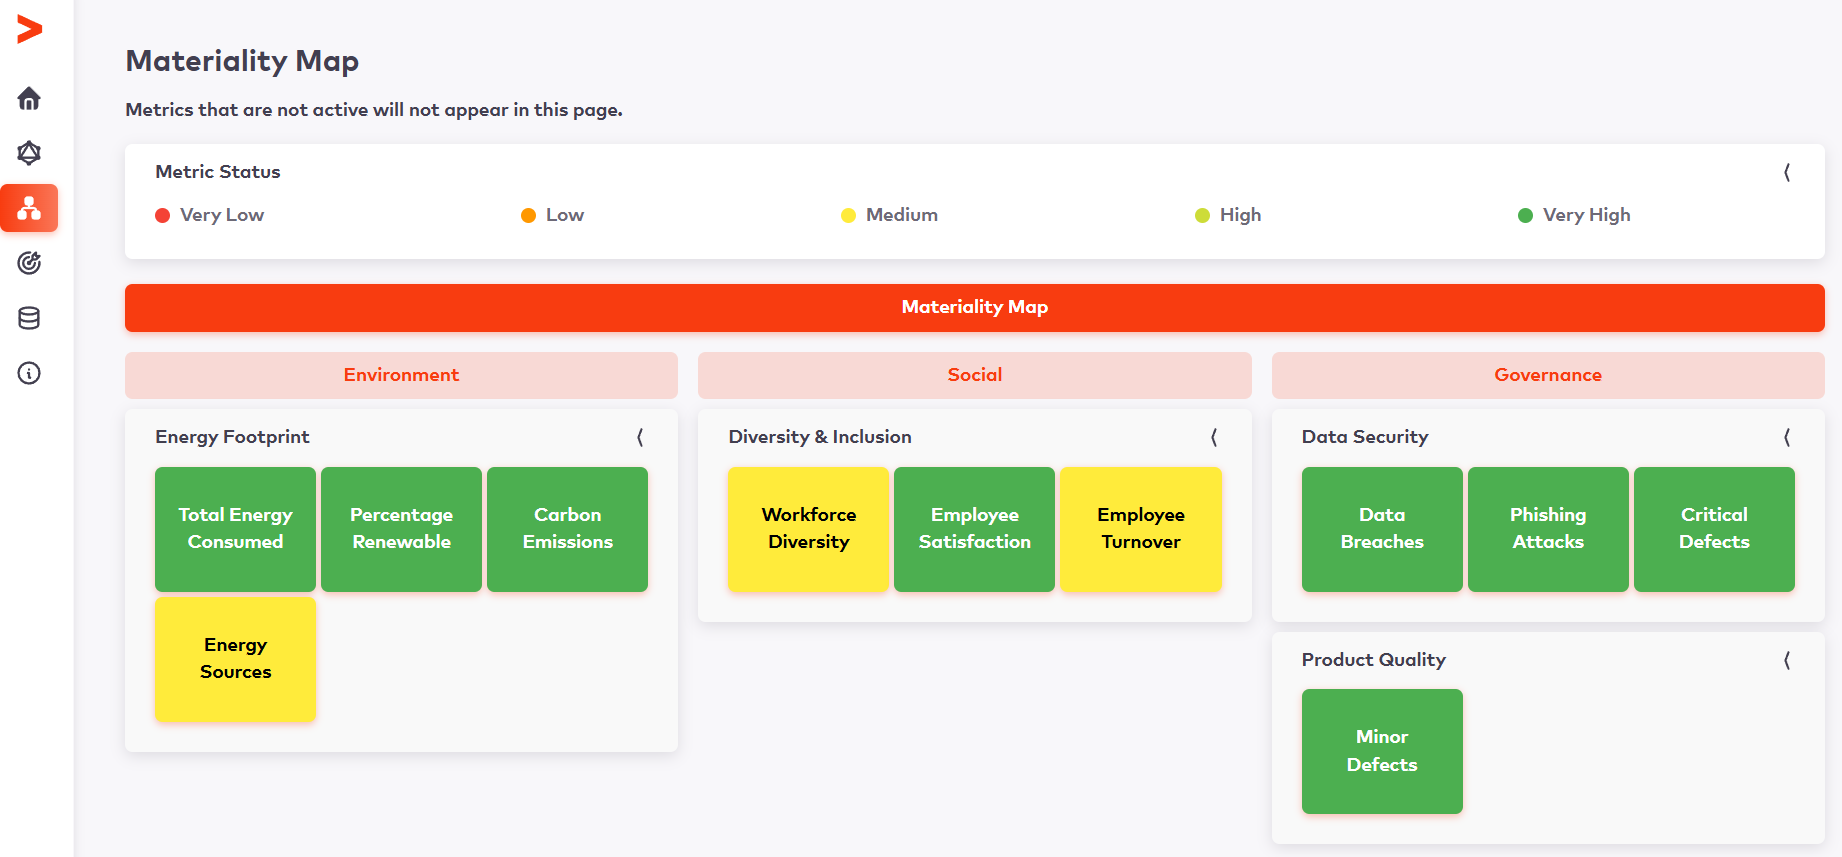
\includegraphics[width=\linewidth,keepaspectratio]{frontmatter/assets/platform_prints/matrix/matrix_done.png}
    \caption{Página da Matriz da Materialidade}
    \label{fig:matrix_done}
\end{figure}

Tal como na página das métricas, cada cartão referente a uma métrica é interativo e disponibiliza a informaçao da mesma, contudo é colorido com base no progresso da métrica associada. A Listagem \ref{lst:metric_classification} refere-se à função responsável por classificar o progresso da métrica e atribuir uma cor correspondente.

\begin{lstlisting}[style=customts, caption={Função de Classificação de Progresso de uma Métrica}, label={lst:metric_classification}]
export function getMetricDevelopmentStatus(
  valueHistories: MetricValueHistory[],
  goalIsDecrease: boolean,
  options = { recentPoints: 5 }
): { status: MetricStatus; color: string } {
  if (valueHistories.length < 2) {
    return { status: 'Medium', color: nodeColors['Medium'] };
  }
  const normalizedHistories = valueHistories.map(h => ({
    ...h,
    recordedAt: new Date(h.recordedAt),
  }));
  const sortedHistories = normalizedHistories.sort(
    (a, b) => a.recordedAt.getTime() - b.recordedAt.getTime()
  );

  const recentHistories = sortedHistories.slice(-options.recentPoints);
  const firstValue = recentHistories[0].value;
  const lastValue = recentHistories[recentHistories.length - 1].value;
  const delta = lastValue - firstValue;
  const adjustedDelta = goalIsDecrease ? -delta : delta;
  const pctChange = (adjustedDelta / firstValue) * 100;

  if (pctChange >= 10) return { status: 'Very High', color: nodeColors['Very High'] };
  if (pctChange >= 5) return { status: 'High', color: nodeColors['High'] };
  if (pctChange > -5) return { status: 'Medium', color: nodeColors['Medium'] };
  if (pctChange > -10) return { status: 'Low', color: nodeColors['Low'] };
  
return { status: 'Very Low', color: nodeColors['Very Low'] };
}
\end{lstlisting}

\subsection{Página dos Conjuntos de Dados}

Cada métrica tem o seu conjunto de dados associado, estando estes acessiveis noutra página da plataforma (Figura \ref{fig:dataset_done}), organizados como entradas numa tabela.

\begin{figure}[H]
    \centering
    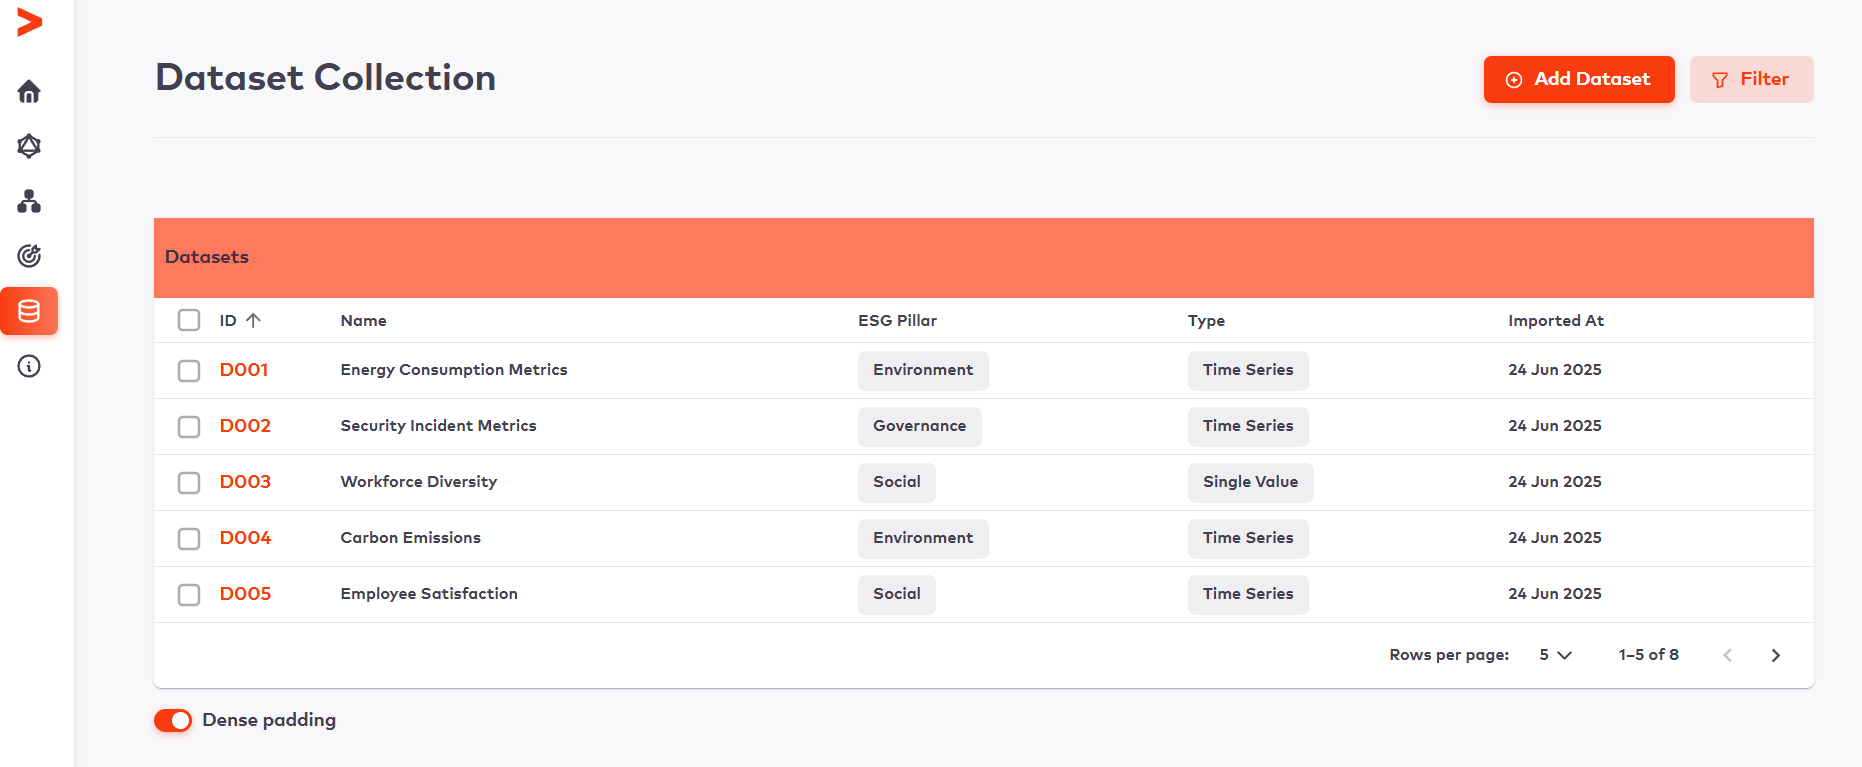
\includegraphics[width=\linewidth,keepaspectratio]{frontmatter/assets/platform_prints/dataset/dataset_done.png}
    \caption{Página dos Conjuntos de Dados}
    \label{fig:dataset_done}
\end{figure}

É nesta página que se observa a implementação do caso de uso UC-07 (Importação de Dados), através de uma janela ilustrada na Figura \ref{fig:create_dataset}, onde são solicitadas as informações necessárias, incluindo o ficheiro CSV que contém os dados. Consoante a estrutura do ficheiro, a interface apresenta diferentes visualizações do mesmo conjunto de dados sob a forma de vários tipos de diagramas. Compete ao utilizador selecionar o tipo de diagrama que melhor representa a informação.

\begin{figure}[H]
    \centering
    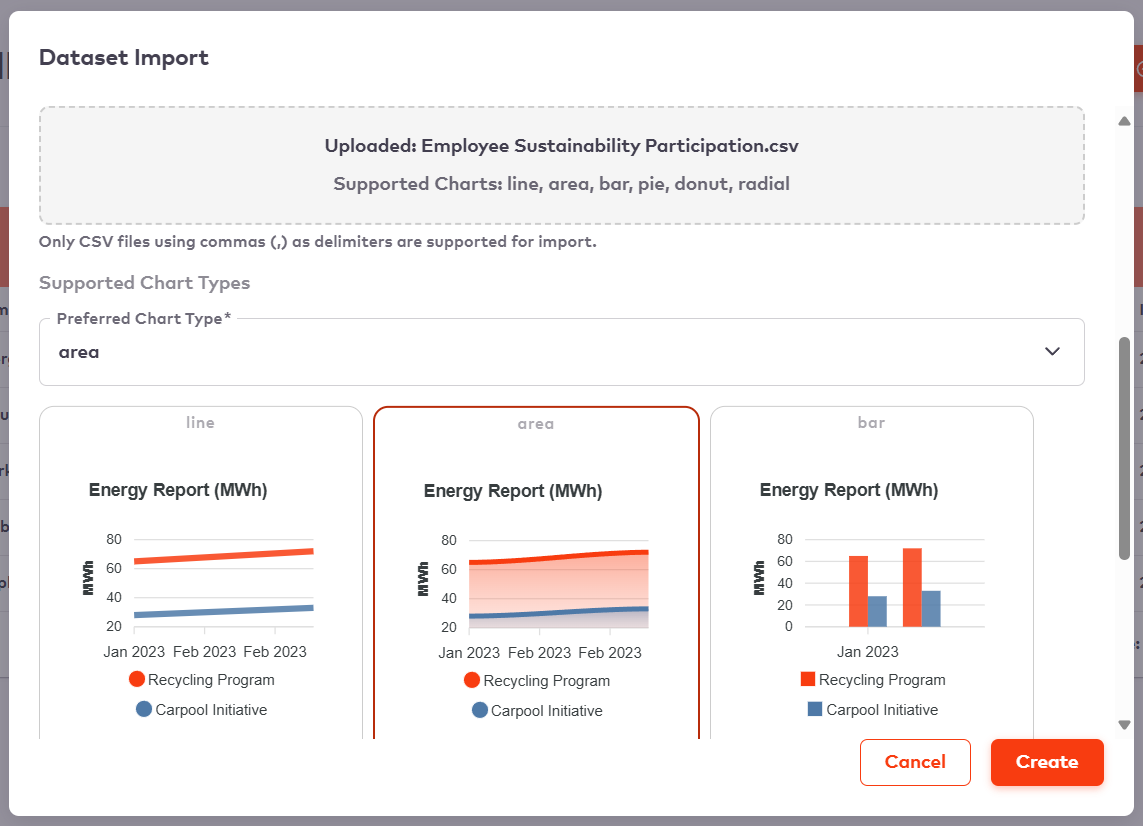
\includegraphics[width=4in,keepaspectratio]{frontmatter/assets/platform_prints/dataset/dataset_import.png}
    \caption{Formulário de Importação de um Conjunto de Dados com Múltipla Renderização de Diagramas}
    \label{fig:create_dataset}
\end{figure}

Após o preenchimento do formulário de importação de dados, é realizado um pedido HTTP do tipo \textit{POST} através da função \texttt{fetch}, com o objetivo de enviar a informação inserida para a rota da API correspondente. A informação submetida é convertida em formato \textit{JSON} e enviada no corpo do pedido, tal como ilustrado na Listagem \ref{lst:import_dataset_api}.

\begin{lstlisting}[style=customts, caption={Chamada à API de Importação de um Conjunto de Dados}, label={lst:import_dataset_api}]
    const response = await fetch('/api/datasets', {
    method: 'POST',
    headers: { 'Content-Type': 'application/json' },
    body: JSON.stringify(newDataset)
    })

    if (!response.ok) {
    const text = await response.text()
    throw new Error(`Failed to import dataset: ${text}`)
    }
    
    const createdDataset: DatasetReadable = await response.json()
\end{lstlisting}

A página permite ainda fazer a filtragem dos conjuntos de dados (Figura \ref{fig:dataset_filter}) mediante o pilar ESG a que estão associados e à sua tipologia.

\begin{figure}[H]
    \centering
    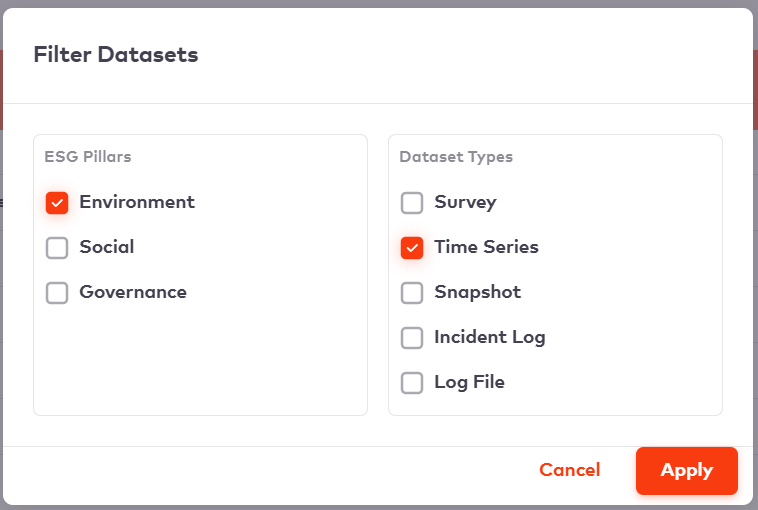
\includegraphics[width=4.5in,keepaspectratio]{frontmatter/assets/platform_prints/dataset/dataset_filter.png}
    \caption{Filtragem de Conjunto de Dados}
    \label{fig:dataset_filter}
\end{figure}

A Listagem \ref{lst:filter_function} apresenta a função que faz o pedido \texttt{GET} onde são aplicados os filtros aos conjuntos de dados com base nos parâmetros definidos na \textit{query url}.

\begin{lstlisting}[style=customts, caption={Função de Filtragem de Conjunto de Dados}, label={lst:filter_function}]
const handleApplyFilters = async (filters: { pillars: string[], types: string[] }) => {
    const queryParams = new URLSearchParams()

    filters.pillars.forEach(pillar => queryParams.append('pillars', pillar))
    filters.types.forEach(type => queryParams.append('types', type))

    const response = await fetch(`/api/datasets/filter?${queryParams.toString()}`, {
      method: 'GET',
      headers: {
        'Content-Type': 'application/json'
      }
    })

    if (!response.ok) {
      console.error('Error fetching filtered datasets')
      return
    }

    const data = await response.json()
    setDatasets(data)
  }
\end{lstlisting}


É ainda possível visualizar a informação de cada conjunto de dados, o seu conteúdo e alternar entre renderizações de diferentes tipos de diagramas, como ilustrado na Figura \ref{fig:dataset_info}.

\begin{figure}[H]
    \centering
    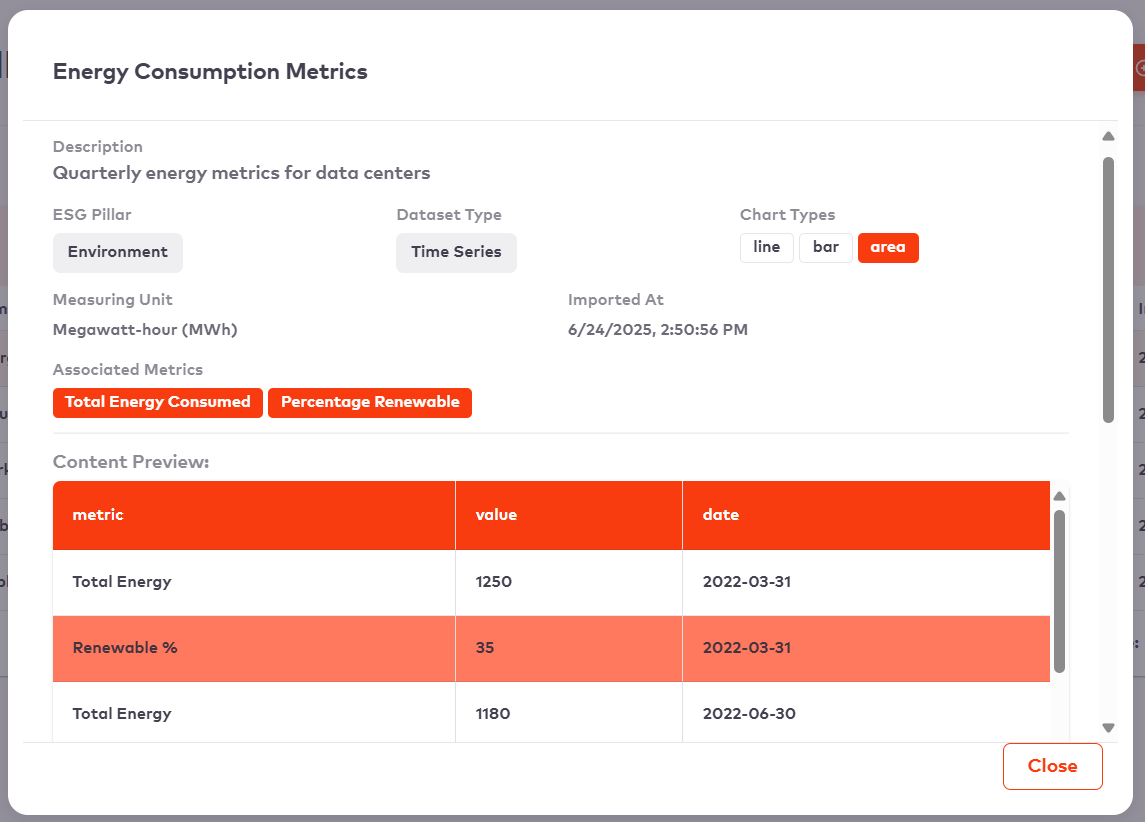
\includegraphics[width=5.5in,keepaspectratio]{frontmatter/assets/platform_prints/dataset/dataset_info.png}
    \caption{Informação de um Conjunto de Dados}
    \label{fig:dataset_info}
\end{figure}

\subsection{Página dos Objetivos}

Esta página da plataforma, ilustrada na Figura \ref{fig:objectives_done}, complementa os casos de uso definidos no projeto, tendo sido desenvolvida por iniciativa da empresa. Na parte superior, apresenta um resumo do estado dos objetivos, indicando quantos foram concluídos, quantos permanecem por cumprir, a percentagem que revela bom progresso e a percentagem que se encontra fora do ritmo esperado.

\begin{figure}[H]
    \centering
    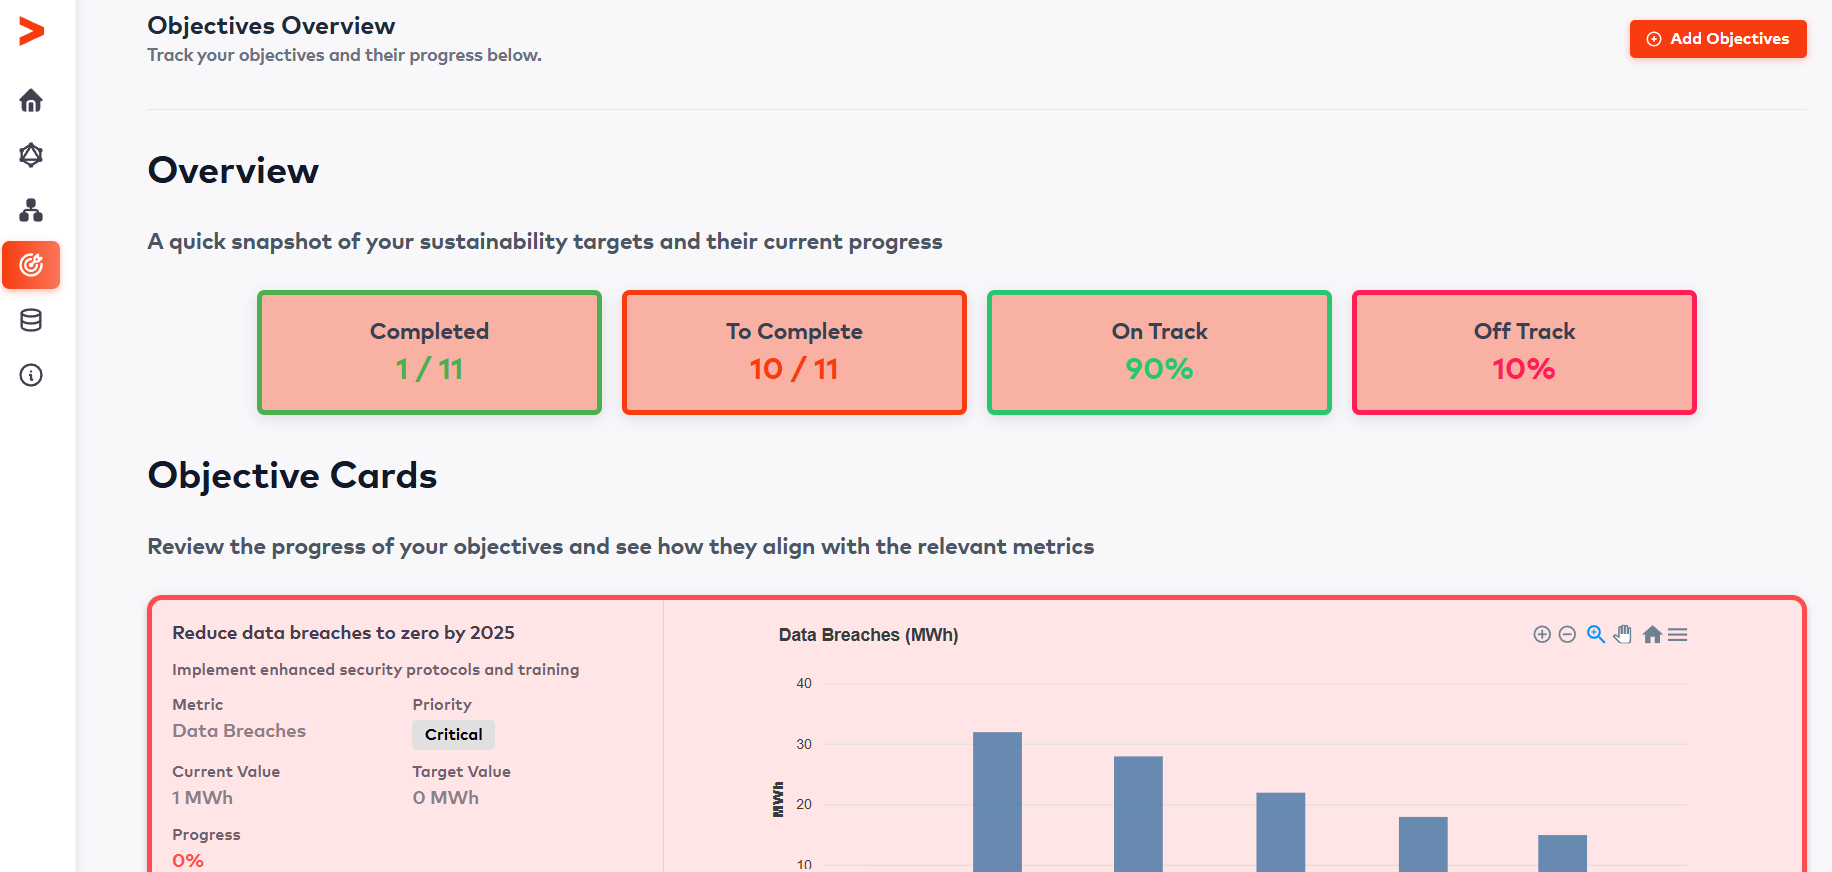
\includegraphics[width=\linewidth,keepaspectratio]{frontmatter/assets/platform_prints/objetives/objective_done.png}
    \caption{Página de Gestão de Objetivos}
    \label{fig:objectives_done}
\end{figure}

A funcionalidade principal desta página é a criação e acompanhamento de objetivos associados a métricas, bem como a avaliação do seu progresso. Cada objetivo é representado num cartão individual, Figura \ref{fig:objective_card}, onde se apresentam as respetivas informações, o nível de progresso e um gráfico com os dados correspondentes. Estes cartões são organizados por ordem de prioridade ou importância atribuída ao objetivo.

\begin{figure}[H]
    \centering
    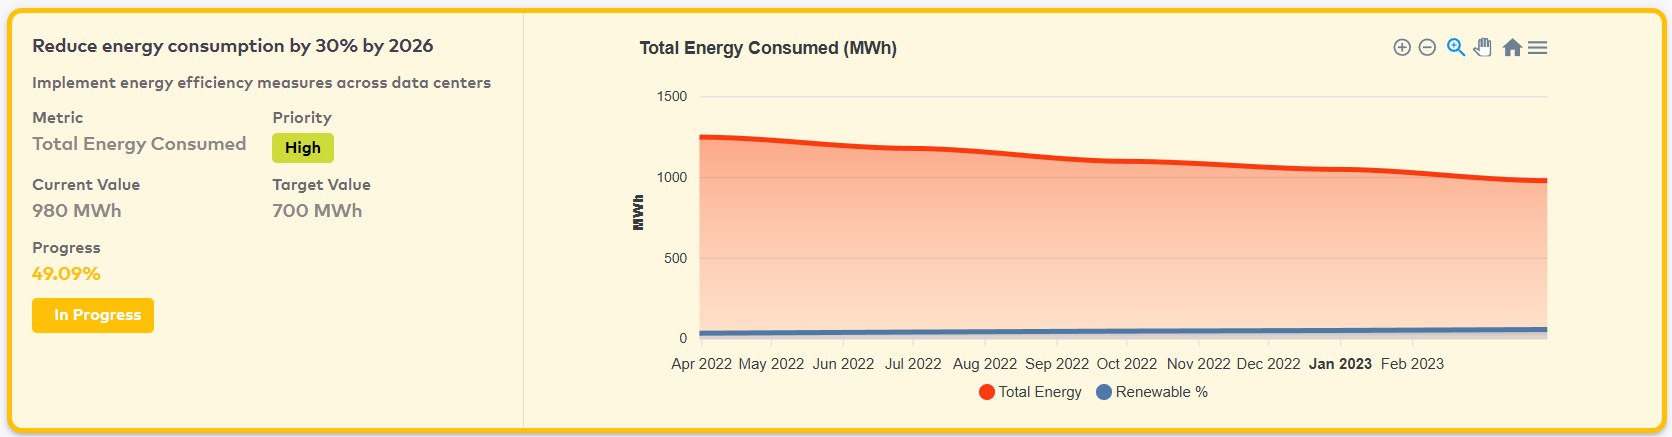
\includegraphics[width=\linewidth,keepaspectratio]{frontmatter/assets/platform_prints/objetives/objective_card.png}
    \caption{Cartão com Informação Detalhada de um Objetivo}
    \label{fig:objective_card}
\end{figure}

A criação de um novo objetivo é iniciada com a submissão de um formulário, que desencadeia um pedido \texttt{POST} à API responsável por registar o objetivo. O envio dos dados é feito em formato \texttt{JSON}, e a resposta da API é validada para garantir o sucesso da operação. Em caso de erro, é apresentada uma mensagem informativa, como indicado na Listagem \ref{lst:create_objective}.

\begin{lstlisting}[style=customts, caption={Pedido \texttt{POST} para criar um novo Objetivo}, label={lst:create_objective}]
const response = await fetch('/api/objectives', {
  method: 'POST',
  headers: { 'Content-Type': 'application/json' },
  body: JSON.stringify(data),
});
if (!response.ok) {
  const errorText = await response.text();
  throw new Error(`Failed to create new objective: ${errorText}`);
}
const createdObjective = await response.json() as ObjectiveReadable;
\end{lstlisting}

O formulário criado para a criação de novos objetivos é ilustrado pela Figura \ref{fig:objective_creation}.

\begin{figure}[H]
    \centering
    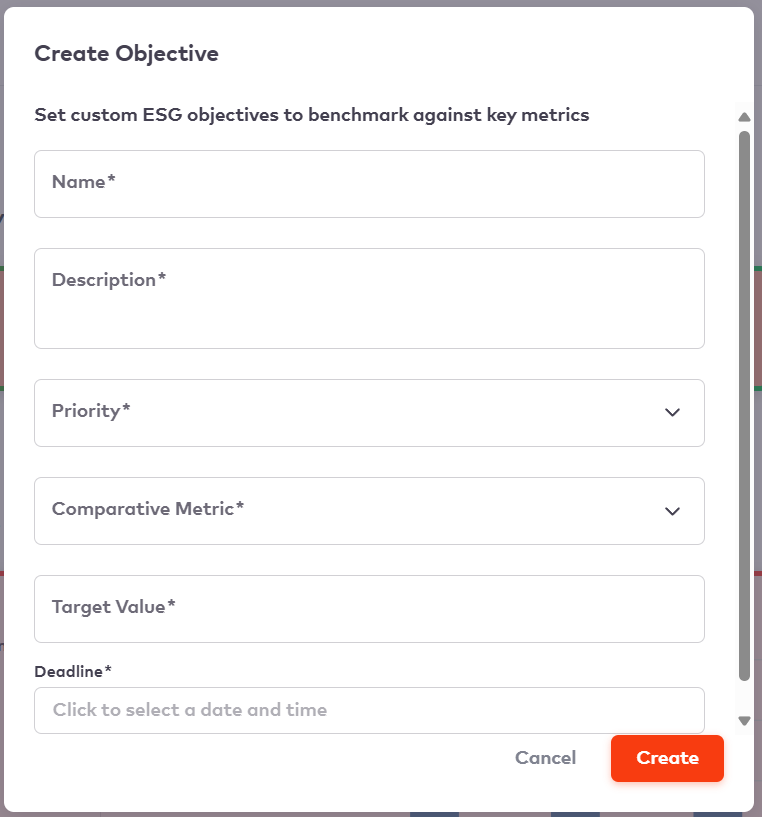
\includegraphics[width=3.5in,keepaspectratio]{frontmatter/assets/platform_prints/objetives/objective_creation.png}
    \caption{Formulário de Criação de Objetivo}
    \label{fig:objective_creation}
\end{figure}

\section{\textit{Seeding} da Base de Dados}

De forma a tornar a demonstração da plataforma mais rica e realista, foram desenvolvidos diversos \textit{scripts} para preparar o estado da base de dados. Estes \textit{scripts} permitem simular diferentes cenários de utilização e facilitar a visualização dos resultados obtidos no \textit{dashboard}.

Inicialmente, foi criado um \textit{script} de limpeza (Listagem \ref{lst:clean_script}) responsável por remover todos os registos existentes na base de dados. Este processo garante que o ambiente de demonstração começa sempre num estado limpo e previsível, evitando interferência de dados anteriores.

\begin{lstlisting}[style=customts, caption={\textit{Script} de limpeza da Base de Dados}, label={lst:clean_script}]
const prisma = new PrismaClient()

async function clearDatabase() {
  console.log('Clearing database...')

  await prisma.objective.deleteMany({})
  await prisma.metric.deleteMany({})
  await prisma.subarea.deleteMany({})
  await prisma.dataset.deleteMany({})
  await prisma.measureUnit.deleteMany({})
  await prisma.pillar.deleteMany({})
  await prisma.company.deleteMany({})
  await prisma.sector.deleteMany({})

  console.log('Database cleared!')
}

clearDatabase()
  .catch(e => {
    console.error('Error clearing database:', e)
    process.exit(1)
  })
  .finally(async () => {
    await prisma.$disconnect()
  })
\end{lstlisting}


De seguida, foi implementado um \textit{script} principal de \textit{seeding} (Listagem~\ref{lst:seeding_script}) que permite popular a base de dados com dados simulados, com base num cenário definido através da variável de ambiente \verb|SEED_SCENARIO|. Este parâmetro pode assumir os valores \verb|good|, \verb|bad| ou \verb|random|, correspondendo a diferentes perfis de desempenho ESG.

\begin{lstlisting}[style=customts, caption={\textit{Script} de \textit{seeding} da Base de Dados}, label={lst:seeding_script}]
const prisma = new PrismaClient()
const SEED_SCENARIO = process.env.SEED_SCENARIO || 'random'

async function main() {
  if (SEED_SCENARIO === 'good') {
    console.log('Seeding good scenario...')
    await seedGood(prisma)
  } else if (SEED_SCENARIO === 'bad') {
    console.log('Seeding bad scenario...')
    await seedBad(prisma)
  } else {
    console.log('Seeding random scenario...')
    await seedRandom(prisma)
  }
}

main()
  .catch(e => {
    console.error(e)
    process.exit(1)
  })
  .finally(async () => {
    await prisma.$disconnect()
  })
\end{lstlisting}

Ao executar o \textit{script}, o cenário selecionado determina qual das funções de \textit{seeding} será invocada: \texttt{seedGood}, \texttt{seedBad} ou \texttt{seedRandom}. Cada uma destas funções é responsável por gerar dados coerentes com o respetivo perfil, permitindo avaliar o comportamento da aplicação em contextos contrastantes.

A geração de dados no cenário aleatório é auxiliada pela biblioteca \texttt{Faker}\footnote{Site oficial do Faker: \url{https://fakerjs.dev/}}, utilizada para criar valores credíveis e variados para simular empresas, métricas e valores ESG. Esta abordagem facilita a demonstração da plataforma e permite observar os efeitos de diferentes perfis de dados no \textit{dashboard}.

A Figura \ref{fig:good_esg} demonstra a pontuação ESG resultante da execução do \textit{script seedGood}.

\begin{figure}[H]
    \centering
    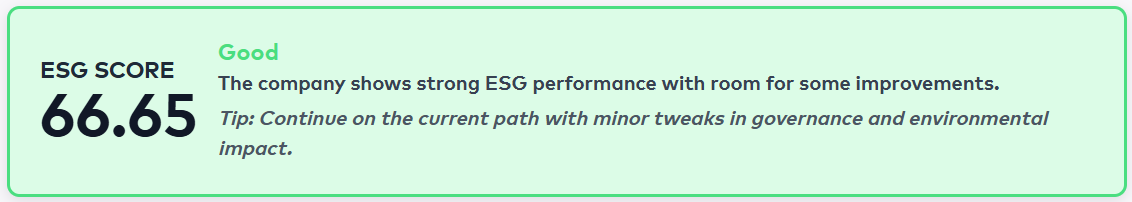
\includegraphics[width=\linewidth,keepaspectratio]{frontmatter/assets/platform_prints/seeding/good_esg.png}
    \caption{Pontuação ESG segundo o \textit{script seedGood}}
    \label{fig:good_esg}
\end{figure}

A Figura \ref{fig:bad_esg} demonstra a pontuação ESG resultante da execução do \textit{script seedBad}.

\begin{figure}[H]
    \centering
    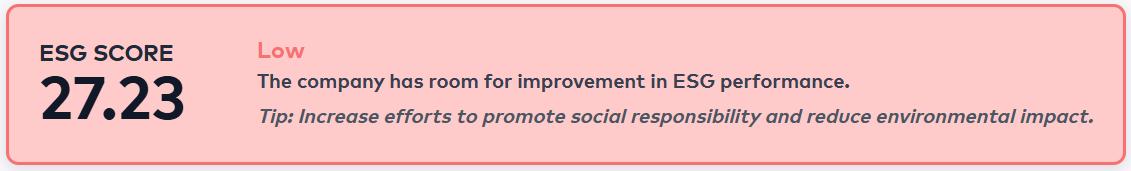
\includegraphics[width=\linewidth,keepaspectratio]{frontmatter/assets/platform_prints/seeding/bad_esg.png}
    \caption{Pontuação ESG segundo o \textit{script seedBad}}
    \label{fig:bad_esg}
\end{figure}

A pontuação ESG resultante da execução do \textit{script} \texttt{SeedRandom} varia significativamente, de forma a simular empresas com diferentes níveis de desempenho em cada um dos pilares ESG: \textit{Environment}, \textit{Social} e \textit{Governance}. Cada valor é atribuído aleatoriamente dentro de um intervalo entre 0 e 100, sendo posteriormente classificado numa das categorias predefinidas: \textit{Very Low} (0--20), \textit{Low} (21--40), \textit{Medium} (41--60), \textit{Good} (61--80), \textit{Great} (81--90) e \textit{Very High} (91--100).

Estas categorias não só representam a qualidade geral da performance ESG da empresa, como também influenciam a forma como os dados são apresentados no \textit{frontend} da aplicação, através de diferentes cores, textos e recomendações visuais para cada cenário. Esta abordagem contribui para uma demonstração mais realista da plataforma, permitindo visualizar comportamentos distintos consoante o perfil ESG simulado.

A Tabela~\ref{tab:esg_categories} resume os intervalos e significados associados a cada categoria.

\begin{table}[H]
    \renewcommand{\arraystretch}{1.3}
    \setlength{\tabcolsep}{10pt}
    \centering
    \begin{tabular}{>{\bfseries}p{2.5cm} p{3cm} p{9cm}}
        \rowcolor{red!30} 
        Very Low & [0--20] & A empresa necessita de melhorias significativas nas suas práticas ESG. \\
        \rowcolor{orange!40} 
        Low & [21--40] & Há margem de progressão, especialmente nas áreas de responsabilidade social e sustentabilidade ambiental. \\
        \rowcolor{yellow!40} 
        Medium & [41--60] & A empresa está no caminho certo, mas ainda precisa de melhorias substanciais. \\
        \rowcolor{green!30} 
        Good & [61--80] & A empresa apresenta um bom desempenho ESG, com espaço para ajustes menores. \\
        \rowcolor{green!45!blue!25} 
        Great & [81--90] & A empresa destaca-se nas práticas ESG, estando próxima da excelência. \\
        \rowcolor{teal!40} 
        Very High & [91--100] & A empresa é uma referência no desempenho ESG e serve como modelo de boas práticas. \\
    \end{tabular}
    \caption{Categorias de pontuação ESG}
    \label{tab:esg_categories}
\end{table}


\section{Testes}

O objetivo dos testes de software é garantir a qualidade do produto, confirmando a sua funcionalidade, desempenho e conformidade com os requisitos previamente estabelecidos (\cite{softdesing2025}). Estes foram realizados com o auxílio do \textit{Jest}\footnote{Site oficial do \textit{Jest}: \url{https://jestjs.io/}} e da \textit{React Testing Library}\footnote{Site oficial da \textit{React Testing Library}: \url{https://testing-library.com/docs/react-testing-library/intro/}}.

Para garantir a robustez e o correto funcionamento da solução desenvolvida, foram concebidos testes de várias tipologias. Foram utilizados testes unitários para garantir que cada componente isolado se comportava como esperado e que as suas funções estavam funcionais. A Listagem \ref{lst:unit_test} refere-se a um teste unitário feito ao componente \texttt{SwiperControls}, na página inicial da aplicação, que verifica o comportamento do componente mediante um cenário onde não existem KPIs válidos.

\begin{lstlisting}[style=customts, caption={Teste unitáro ao componente \texttt{SwiperControls}}, label={lst:unit_test}]
it('renders a message when no valid KPIs exist', () => {
    const noHistoryMetric: MetricInfoCard = {
      ...baseMetric,
      valueHistories: []
    }
    render(<SwiperControls kpis={[noHistoryMetric]} />)
    expect(screen.getByText(/no metrics with sufficient history/i)).toBeInTheDocument()
  })
\end{lstlisting}

Paralelamente, foram realizados testes de integração com o objetivo de verificar a comunicação e interação entre os vários componentes e confirmar que estes funcionam de forma harmoniosa e consistente quando combinados. Um teste de integração entre os componentes \texttt{ChartErrorBoundary} e \texttt{ChartRenderer} é apresentado na Listagem \ref{lst:integration_test}. De forma a evitar que a aplicação falhe completamente, o componente \texttt{ChartErrorBoundary} é responsável por capturar os erros ocorridos durante a renderização dos gráficos no seu componente de ficheiro, neste caso o \texttt{ChartRenderer}. Adicionalmente, assegura o registo das mensagens de erro (\textit{logging}), permitindo uma melhor monitorização e diagnóstico do problema.

\begin{lstlisting}[style=customts, caption={Teste de integração entre o componente \texttt{ChartErrorBoundary} e \texttt{ChartRenderer}}, label={lst:integration_test}]
describe('ChartErrorBoundary + ChartRenderer integration', () => {
    it('renders fallback UI when ChartRenderer throws due to invalid dataset', () => {
        const invalidDataset = {
            headers: ['value'], // falta a informacao das datas dos registos
            rows: [
                { value: 42 },
                { value: 12 }
            ]
        };

        render(
            <ChartErrorBoundary>
                <ChartRenderer
                    chartType="line"
                    dataset={invalidDataset}
                    datasetType="Time Series"
                    title="Invalid Test Chart"
                    unit="kg"
                />
            </ChartErrorBoundary>
        );

        expect(screen.getByText(/missing required date field/i)).toBeInTheDocument();
    });
});
\end{lstlisting}

Esta abordagem diversificada leva à criação de um elevado número de testes, Figura \ref{fig:test_number}, permite identificar falhas a vários níveis do sistema, o que contribui para melhorar a qualidade contínua e a qualidade do produto final.

\begin{figure}[H]
    \centering
    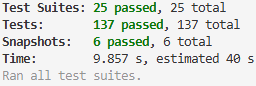
\includegraphics[width=2.5in,keepaspectratio]{frontmatter/assets/tests/test_suits.png}
    \caption{Testes desenvolvidos para a solução}
    \label{fig:test_number}
\end{figure}

A Figura \ref{fig:coverage} ilustra o resumo do relatório de cobertura dos testes desenvolvidos. 

\begin{figure}[H]
    \centering
    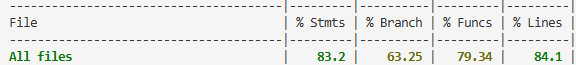
\includegraphics[width=\linewidth,keepaspectratio]{frontmatter/assets/tests/coverage.png}
    \caption{Resumo do relatório de cobertura dos testes desenvolvidos da solução}
    \label{fig:coverage}
\end{figure}

Estes valores mostram um grau razoável de testes automatizados, especialmente na execução de instruções e cobertura de linhas, com alguma margem para melhoria na cobertura de ramos, para ajudar a garantir que todas as vias lógicas são adequadamente testadas.

\section{Avaliação da solução} 

A aplicação apresenta tempos de carregamento eficientes, não ultrapassando os 30 segundos por página, como se pode ver na Figura \ref{fig:page_compiling}, o que cumpre os critérios definidos para o projeto.

\begin{figure}[H]
    \centering
    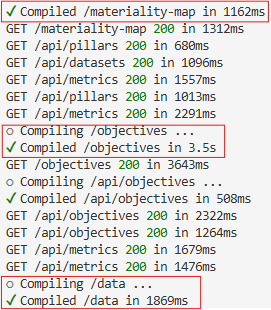
\includegraphics[width=2.5in,keepaspectratio]{frontmatter/assets/compiling/pages_time.png}
    \caption{Compilação das páginas em menos de 30 segundos}
    \label{fig:page_compiling}
\end{figure}

Para verificar se o tempo total de carregamento da solução idealizada, incluindo tanto o processo de \textit{seeding} da base de dados quanto a compilação da página inicial, estava dentro do intervalo de 3 minutos, foi criado um \textit{script} especial, como pode ser observado na Listagem \ref{lst:eval_script}.

\begin{lstlisting}[style=customts, caption={\textit{Script} de avaliação de performance da iniciação da aplicação desenvolvida}, label={lst:eval_script}]
#!/bin/bash

echo "Seeding and setup started at: $(date '+%Y-%m-%d %H:%M:%S')"
START=$(date +%s)

npm run db:soft-reset
npm run seed:good

END=$(date +%s)
echo "Seeding and setup ended at: $(date '+%Y-%m-%d %H:%M:%S')"
echo "Duration: $((END - START)) seconds"

echo "Now starting the dev server..."
npm run dev
\end{lstlisting}

A Figura \ref{fig:initial_compile} mostra o resultado obtido com a execução deste \textit{script}, confirmando o cumprimento do requisito avaliado e evidenciando um tempo de compilação inicial de 49,5 segundos.

\begin{figure}[H]
    \centering
    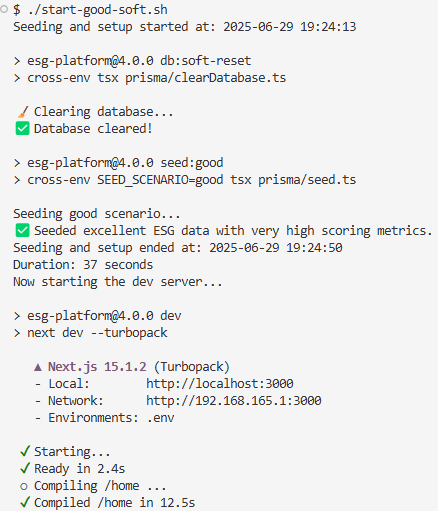
\includegraphics[width=3.5in,keepaspectratio]{frontmatter/assets/compiling/initial_compile.png}
    \caption{Execução do \textit{script} de avaliação do tempo de compilação inicial}
    \label{fig:initial_compile}
\end{figure}

As animações utilizadas são fornecidas pelos componentes nativos do \textit{React} e pelo template \textit{Vuexy}, para uma experiência visual contínua e suave, sem sacrificar o desempenho da aplicação.

O design da aplicação é de fácil utilização e foi elogiado por várias partes interessadas, tais como o supervisor de estágio, o \textit{buddy} (colaborador responsável pelo acompanhamento do estagiário na empresa), a equipa de produtos DevScope, que também analisou o protótipo apresentado no Apêndice \ref{AppendixC}, bem como colegas da universidade e do estágio. A navegação foi clara e intuitiva, facilitando a interação dos utilizadores com o sistema.

Os componentes implementados atendem ao esperado, sem apresentar erros imprevistos ao serem utilizados. O código é organizado em módulos, facilitando alterações e manutenções futuras, fruto não apenas da arquitetura tradicional das aplicações \textit{React}, mas também da aplicação estrita de boas práticas de programação.

No que respeita à acessibilidade, a aplicação tem a língua inglesa e incorpora as cores institucionais da organização. A aplicação destina-se apenas a ser utilizada em computadores, posicionando-se como uma área com espaço para melhorias no futuro.

Foram efectuados testes unitários e testes de integração para garantir a estabilidade e a qualidade do sistema disponível. Além disso, a usabilidade foi testada com a participação de colegas, o que ajudou a revelar possíveis melhorias na experiência do utilizador. Os conjuntos de dados aplicados são imaginários, numa tentativa de manter a confidencialidade da empresa no que respeita às questões ESG abrangidas. A cobertura dos testes é considerada satisfatória, apesar de haver alguma margem para melhorias, nomeadamente em termos de ramos de código.

\section{Implementação Alternativa} 

Durante o processo de desenvolvimento da aplicação, foi tida em conta a utilização de ferramentas de terceiros para complementar ou substituir, em determinadas áreas, componentes da solução desenvolvida. Especificamente, o \textit{Microsoft Power BI} surgiu como uma alternativa que poderia trazer vários benefícios, nomeadamente na visualização de dados, criação de relatórios interactivos e gestão do esquema de dados de forma dinâmica e centralizada. Esta abordagem permitiria que os utilizadores finais pudessem analisar os dados ESG de uma forma mais detalhada e visualmente apelativa, tirando partido de um ecossistema maduro e popular no contexto empresarial.

Esta hipótese ganhou um significado ainda maior à luz do acordo de parceria entre a DevScope e a \textit{Microsoft}, que facilitaria a integração do \textit{Power BI} na estrutura da solução, tanto estratégica como tecnicamente.

No entanto, na sequência de uma análise interna e de uma consulta à equipa de produto, concluiu-se que, relativamente aos objectivos estabelecidos para o projeto, essa abordagem teria inconvenientes consideráveis. A principal consideração a favor de uma solução personalizada foi o modelo de negócio pretendido: a criação de um produto de venda única, independente de subscrições ou licenciamentos contínuos de terceiros. A utilização do \textit{Power BI} obrigaria a que os utilizadores da solução estivessem associados a uma subscrição ativa do serviço por parte da \textit{Microsoft}, o que poderia ser um inibidor de adoção e comprometer a independência da organização relativamente ao produto final. Desta forma, foi determinada a implementação de uma aplicação autónoma, que fornece visualizações personalizadas e permite o controlo total sobre todos os elementos da experiência do utilizador, alinhando-se com os objectivos de negócio da DevScope, bem como com as melhores práticas no desenvolvimento de soluções de negócio escaláveis a nível empresarial.